\documentclass[]{spie}  %>>> use for US letter paper

\newcommand{\docRef}{TSTN-045}
\newcommand{\docUpstreamLocation}{\url{https://github.com/lsst/tstn-045}}

\renewcommand{\baselinestretch}{1.0} % Change to 1.65 for double spacing

\usepackage{amsmath,amsfonts,amssymb}
\usepackage{graphicx}
\usepackage[colorlinks=true, allcolors=blue]{hyperref}

\title{Replacing DDS with Apache Kafka as middleware technology for the Rubin Observatory Control System}
\date{\today}

% This can write metadata into the PDF.
% Update keywords and author information as necessary.
\hypersetup{
    pdftitle={Replacing DDS with Apache Kafka as middleware technology for the Rubin Observatory Control System},
    pdfauthor={ribeirot},
    pdfkeywords={}
}

\input{authors.tex}
\authorinfo{Further author information: (Send correspondence to T.R.)\\T.R.: E-mail: tribeiro@lsst.org, Telephone: 1 520 589 3669}

% Option to view page numbers
\pagestyle{empty} % change to \pagestyle{plain} for page numbers
\setcounter{page}{301} % Set start page numbering at e.g. 301

\begin{document}
\maketitle

\begin{abstract}
Once in operation, the Vera C. Rubin Observatory will execute a 10-year-long survey of the Southern sky known as the Legacy Survey of Space and Time (LSST).
The Rubin Observatory Control System (Rubin-OCS) is a distributed system with each component in charge of a particular sub-system e.g.; the mount, the M1M3 mirror support system, etc.
Each component is designed as an independent part of the system and they must work together during operations.
Communication between the components is done by means of a software middleware.

The software middleware is the backbone of the system, allowing components to communicate with each other in a seamless way.
The highly distributed nature of the Rubin-OCS places tight constraints in terms of latency, availability, and reliability for the middleware.
The baseline implementation of the Rubin-OCS adopts the Data Distribution Service (DDS) technology for the middleware.

In the Rubin-OCS, the middleware is encapsulated with a layer of abstraction known as the Service Abstraction Layer (SAL), which currently uses the ADLink-OpenSpliceDDS implementation of the Data Distribution Service (DDS) message passing system.

Recently we performed a study of using Apache Kafka to replace DDS as the middleware technology for the Rubin-OCS.
This study was motivated by the middleware-related challenges we faced while integrating the system as well as the recent announcements indicating that the adopted library may be deprecated during the lifespan of the project.
The study involved throughput and latency studies and a proof of concept of our core libraries.
Overall Kafka proved to be a suitable replacement for DDS.
\end{abstract}

\keywords{Vera C. Rubin Observatory, observatory control, middleware, Kafka, Data Distribution Service, DDS}

\section{INTRODUCTION}
\label{sec:intro}

Middleware typically denotes software applications utilized for enabling communication in parallel and distributed computing\cite{BUYYA201329}.
This technology became popular with the advent of distributed systems, which come as a solution to the problem of parallel computation.
As software and hardware systems became more complex, it becomes impractical to develop and execute them in a single process and, eventually, a single node.
With that, software evolved from monolithic applications, where a single program executes in a single process or node, to distributed applications, where the system is divided into a number of smaller applications; each running on their own process or node.
For these applications to work together coherently they must be able to communicate with each other, thus giving origin to middleware technologies.

How a distributed system is broken down into smaller pieces is heavily dependent upon the problem.
Some systems are only broken down into a small number of components each still in charge of large contexts, others are broken down into many small applications that are in charge only of small simple tasks.
The latter has gained substantial popularity recently and is commonly referred to as \textit{microservices}.
These systems are behind many of popular large services in use today like Google and Amazon.

The architecture of distributed systems can take many shapes and forms.
For instance, some systems are designed to emulate monolithic applications.
The application is composed of a number of smaller applications but there is a hierarchical organization, with components at the top, in charge of communicating and operating components at the bottom.
The advantage of these systems is that they are easier to understand and to maintain.
Since each component is isolated from the rest of the system, and only communicates with a components on the top and bottom of the hierarchical chain, adding new components is relatively easy and have minimal impact in the system.
The disadvantage is that the system is more vulnerable to outages, if a component on the top of the hierarchical chain becomes unavailable those components at the bottom also become unavailable.

More modern distributed systems have been favoring less hierarchical approaches, following the principles of reactive systems.
In these systems each component is designed as an independent entity that reacts to input data, be it from other components or external data services.
Since these systems are designed with separation of concerns in mind (e.g. each component must be able to act independently), reactive systems are usually extremely resilient.
If one component becomes unavailable, the others are expected to continue to operate, taking precautions to deal with the missing agent.
At the same time, it can become quite burdensome to update and grow these systems as their complexity increases exponentially with the number of different components.

In any case, the middleware plays a crucial role in any kind of distributed system, acting as the glue that binds the system together.

The Vera C. Rubin Observatory\cite{2019ApJ...873..111I} Control System (Rubin-OCS) is designed following the principles of a distributed, reactive architecture.
The system is composed of a number of independent components that work together to execute cohesive operations.
The middleware is encapsulated with a layer of abstraction known as the Service Abstraction Layer (SAL), which currently uses the ADLink-OpenSpliceDDS implementation of the Data Distribution Service (DDS) message passing system \cite{2010SPIE.7740E..2CM}.
Like similar projects before us\cite{10.1117/12.2313106}, we experienced considerable challenges with DDS while rolling out the system into production.
While we were able to resolve the majority of those issues by fine tuning ADLink-OpenSpliceDDS configuration, a number of recurrent issues still remain, which are hard to track down and resolve due to their non-repeatable nature.
However, one of the most critical aspects, that inspired us to look for a replacement is that the adopted library is currently bound for sunsetting.

With all that in mind we decided to explore alternative solutions for the Rubin-OCS.
After exploring a number of alternatives, we decided to adopt Kafka as the message passing system, with AVRO-schema encoding for the topics schema.

In the following sections we describe the work done to validate the adoption of Kafka and the initial results obtained with the system running in one of our test stands.
In Section~\ref{sec:comparison} we provide a comparison between DDS and Kafka in the context of the Rubin-OCS, including a description of their similarities, differences and a performance review.
In Section~\ref{sec:swd} we describe our initial experience deploying the full system on a test stand, followed by conclusions in Section~\ref{sec:conclusions}.

\section{Comparison between DDS and Kafka}
\label{sec:comparison}

In this section we present a comparison between DDS and Kafka in the context of the Rubin-OCS.

\subsection{Similarities}
\label{subsec:similarities}

One of the main similarities between DDS and Kafka, which weighted considerably when we decided to explore Kafka as a viable replacement, is the fact that both use a publish-subscribe model to transmit and receive messages.
Each message is associated with a “topic”, which can be understood as a communication channel to exchange a particular type of message.

In both cases, the message transport happens over TCP/IP protocol.

Both DDS and Kafka have support for durability, which is the capability to retrieve historical data (often referred to as “late-joiner”), and our control system architecture relies heavily on this feature.
As a node starts up, it reads the most recent historical message for each event it subscribes to in order to get the current state of the system, without having to resort to requesting information to be republished.

% However, we do not read historical data for commands, because reponding to stale commands is dangerous.
% We also do not read historical telemetry because telemetry is output frequently, so there is no need, and we want to be sure it the data is current.

\subsection{Differences}
\label{subsec:differences}

One of the main distinctions between these two systems is that Kafka is brokered, whereas DDS is distributed, with no central broker.

With DDS each node discovers the other nodes, using UDP multicast, as the application starts up.
Durability is achieved by the election of a main node which stores all the historical data and distributes them as needed, switching which node acts as the primary source of data if one fails.

With Kafka each node connects to a broker (and schema registry); there is no discovery phase and no need for UDP multicast.
Kafka writers write messages to the broker, and readers read messages from the broker.
This is a much simpler topology than DDS, but it does require that each message be sent to the broker and then again to each subscriber, which may result in increased latency.
Durability is a natural attribute of the system as the brokers store messages for distribution by design.
Reliability and performance can be increased by running multiple brokers in parallel, and by using more than one partition for each topic.

\subsubsection{Topic Schema and Schema Evolution}
\label{subsubsec:schema_evolution}

In DDS each individual topic has a specific pre-defined schema.
In the specification that we are using, DDS does not support schema evolution.
This means that, once a topic is created all further readers and writers must have the same topic schema.
Thus, in order to prevent collisions between old topic schemas and new topic schemas, we include a hash to the topic name that changes whenever the schema changes.
Our high-level software hides that hash from users.
Although this helps us avoid schema collisions in the running system, this causes silent errors if systems are brought up with different topic schemas.
We have managed to avoid this issue by enforcing a tight deployment procedure that guarantees all systems are running with the same schema version.

Kafka topics on their own have no concept of schema, working more like a communication channel than as a specific message exchange.
However, Kafka ships with a schema register that can be used to register and validate topic schema.
The schema register can be configured with different levels of support for schema evolution and supports a variety of schema specifications.
For the Rubin-OCS we adopted AVRO-schema, in part because it was already in use in the project but also because it provides great level of flexibility.
For the time being we have only made limited use of all the capabilities provided by an advanced schema evolution mechanism.
In the future we expect to be able to allow systems to update their interfaces more freely, considerably improving the timeline to deploy new features to the system.

\subsubsection{Subtle Differences Between DDS and Kafka}
\label{subsubsec:subtle_differences}

DDS topics have the concept of “quality of service” (QoS) settings for topics.
There are many QoS settings, and the settings must match quite closely between publishers and subscribers of a particular topic, else the topic cannot be constructed.
This has been a source of much frustration over the years, though we have finally found QoS settings that work.

The settings for publishing Kafka topics are far simpler than for DDS, and subscribers have no settings.
Kafka publishers can specify the number of partitions (increasing the number of partitions increases throughput) and how many ACKs to listen for when writing a message (a tradeoff between latency and reliability).

DDS topics have the concept of “liveness” (one of the many QoS settings), whereas Kafka topics do not.
We have configured our DDS topics such that messages are no longer alive when a CSC exits, in order to avoid collisions between older and newer versions of topic QoS when upgrading control software.
Changes to a topic’s schema are handled by changing a hash field in the DDS topic’s name, as mentioned in Section~\ref{subsubsec:schema_evolution}.
The result is a completely different topic, as far as DDS is concerned.
Until we learned to do this, we frequently ran into a problem where we could not run a new version of a component, because it could not create its topics due to an incompatibility with cached “zombie” data.
But marking topics as dead when an application exits means that historical data for a component that have quit is not unavailable from DDS.

Kafka has no concept akin to “liveness”, neither does it need it.
In most cases we can simply run the new application.
If a topic’s schema has changed in some incompatible way then we might have to clean up the broker and schema registry.

\subsection{Performance}
\label{subsec:performance}

One of our main concerns in adopting Kafka as a replacement for DDS was to ensure its performance was on par with our systems requirements.
Our primary performance requirements are:

\begin{itemize}
  \item Average latency better than 25ms.
  \item Latency standard deviation better than 3ms.
  \item Throughput better than X MB/s per topic.
  \item Consumers must be able to keep up with the data they read.
  \item Must be able to handle the full system throughput.
\end{itemize}

A major aspect of adopting Kafka, is that it is already in use in the DDS-based control system to feed data to the Engineering Facility Database (EFD).
We have been operating the system with this architecture from the very beginning, which allowed us not only to gain experience with Kafka, but also to demonstrate that Kafka is able to handle the load.
Overall, the only aspect we have not investigated is the latency in which messages are delivered from publishes to subscribers.

Thus for measuring performance we concentrated on the first four items.

We tested performance using three topics:

\begin{itemize}
  \item MTM1M3 summaryState: One of the smallest topics.
  \item MTMount trackTarget: The command which we most care about latency.
    This is the command sent by the pointing component to the mount with on sky pointing demands.
    It is this operation that derives the latency values above.
  \item MTM1M3 forceActuatorData: The largest topic in the systems, which is also published at 50Hz.
    This topic sets the per topic throughput requirement.
\end{itemize}

For Kafka we performed the tests using two different settings:

\begin{itemize}
  \item \texttt{ack=0}, meaning the writers will not wait for confirmation from the broker that the topic was received.
    This is not considered safe, and is provided purely to show how much latency is due to waiting for acknowledgement.
  \item \texttt{ack=1}, meaning the writers will wait for 1 acknowledgement from the broker.
    This is a very common configuration that is considered safe.
\end{itemize}

For DDS we used our standard configuration.
All tests were executed on a dedicated node with the same configuration we use for our production environment.

The results are presented in the following sessions.

\subsubsection{Latency}
\label{subsubsec:performance:latency}

Latency was estimated by writing 2000 messages at 20 Hz and measuring the time between when each message was written and when the reading process received that message.
The results are shown in Table~\ref{tab:latency}.

\begin{table}[h]
    \centering
    \begin{tabular}{|c|c|c|c|c|c|c|}
        \hline
        System & ACKs & Topic             & \multicolumn{4}{c|}{Latency (ms)} \\
               &      &                   & mean & stdev & min & max     \\
        \hline
        DDS    & n/a  & summaryState      & 1    & 0     & 1   & 1       \\
        DDS    & n/a  & trackTarget       & 1    & 0     & 1   & 2       \\
        DDS    & n/a  & forceActuatorData & 5    & 0     & 4   & 7       \\
        Kafka  & 0    & summaryState      & 2    & 0     & 2   & 6       \\
        Kafka  & 0    & trackTarget       & 2    & 0     & 2   & 4       \\
        Kafka  & 0    & forceActuatorData & 3    & 0     & 3   & 8       \\
        Kafka  & 1    & summaryState      & 2    & 1     & 2   & 27      \\
        Kafka  & 1    & trackTarget       & 2    & 1     & 2   & 25      \\
        Kafka  & 1    & forceActuatorData & 3    & 0     & 3   & 23      \\
        \hline
    \end{tabular}
    \caption{
      Summary of the latency measurements performed with DDS and Kafka for three different topics.
      For Kafka we performed latency measurements with two different setups; \texttt{ack=0} and \texttt{ack=1}.
      When  \texttt{ack=0} the writer will not wait for confirmation from the broker that the topic was written before proceeding, whereas with  \texttt{ack=1} it will wait for at least 1 receive acknowledgement.
      The three different topics used in this test represents the smallest (summaryState) and the largest (forceActuatorData) topics in our system, plus an intermediary case that requires the lowest latency possible (trackTarget).
    }
    \label{tab:latency}
\end{table}

Latency is only an issue for tracking demands, which are sent at approximately 20 Hz and specify position, velocity, and time.
Tracking demands are presently sent at least 50 ms in advance, so it is possible that an occasional tracking command be late, due to an extreme outlier latency.
This should not be a problem, because our specifications allow us to lose up to three sequential tracking commands, so we can afford to ignore (with a warning) the occasional late command.

We could also send tracking commands a bit farther in advance.
This would decrease the responsiveness to offsets and new slews by the same small amount.

\subsubsection{Write Speed}
\label{subsubsec:performance:speed}

Write speed was measured by having two separate processes, a writer and a reader, writing and reading messages as quickly as possible.
The test executed until the reader had received 10,000 messages.
We decided to use the number of received messages as the stopping point in order to improve metrics in situations where there is data loss.
The results are shown in Table~\ref{tab:speed}.

\begin{table}[h]
    \centering
    \begin{tabular}{|c|c|c|c|c|c|}
        \hline
        System & Acks & Topic             & Write Speed & Read Speed & Messages lost \\
               &      &                   & messages/s  & messages/s &               \\
        \hline
        DDS    & n/a  & summaryState      & 16,553      & 16,580     & 0             \\
        DDS    & n/a  & trackTarget       & 13,557      & 13,577     & 0             \\
        DDS    & n/a  & forceActuatorData &  1,912      &  1,492     & 2,632         \\
        Kafka  & 0    & summaryState      &  4,730      &  4,739     & 0             \\
        Kafka  & 0    & trackTarget       &  4,379      &  4,385     & 0             \\
        Kafka  & 0    & forceActuatorData &  3,267      &  3,262     & 0             \\
        Kafka  & 1    & summaryState      &  2,065      &  2,066     & 0             \\
        Kafka  & 1    & trackTarget       &  1,841      &  1,842     & 0             \\
        Kafka  & 1    & forceActuatorData &  1,652      &  1,652     & 0             \\
        \hline
    \end{tabular}
    \caption{
      Write speed measurements for DDS and Kafka.
      As with the latency measurements in Section~\ref{subsubsec:performance:latency} () the measurements were performed with 2 different configurations for the Kafka writer and for three different topics.
      See Table~\ref{tab:latency} for more details.
    }
    \label{tab:speed}
\end{table}

These throughputs all easily meet our requirements.

Note that, alongside write speed and message loss, we also report read speed.
It is worth noting that this is not a measure of maximum read speed, as this is limited by the write speed.
In general, as long as the reader can keep up with the writer, read speed should be approximately the same as write speed.
It is not clear to us why the reported read speed is sometimes slightly higher than write speed.
We believe that this might be because the writers starts a shortly before the reader and it might have time to write some messages before the readers starts to read them.
This would cause the reader to quickly read messages previously in the historical queue and suggests that it is possible to consume messages faster than we can produce it which is, in general, a desirable property in publish-subscribe systems.

The fact that some DDS messages were lost shows that our DDS testing harness can write large messages faster than it can read them.
This is not a cause for concern, as long as we keep up with the actual rate at which messages are written at operational regimes (e.g. 50Hz).

\section{System Wide Deployment}
\label{sec:swd}

Following the encouraging performance results we obtained with Kafka, we went ahead and started a system-wide adoption project.
We started by updating our high level Python library to replace DDS with Kafka.
During this period we wanted to maintain compatibility between both versions of the library to ease the transition.
Overall, the worked pretty well and we are able to provide a compatible versions of the library that can be seamlessly swapped.

Although the majority of our components are written using the high level Python library, some of the most critical components are written in C++ and Java, namely; the pointing component, the M1M3 support system (both in C++) and the cameras control system (in Java).
The second phase of the process was then to update our C++ and Java components.

Before we can finally run the system at the Summit, driving the observatory systems, we need to ensure it works as expected.
With all our systems able to run with Kafka, we made a full deployment of all the components in one of our Test Stands.
This is possible because all our systems are developed with a simulation mode that closely emulate the actual component behavior.
We regularly use our components in simulation mode on our Test Stands for integration tests and for testing operations before deploying them at the Summit.
In Figure~\ref{fig:swd}, we show a screenshot of the user interface of our system running Kafka.

\begin{figure}[h]
  \centering
  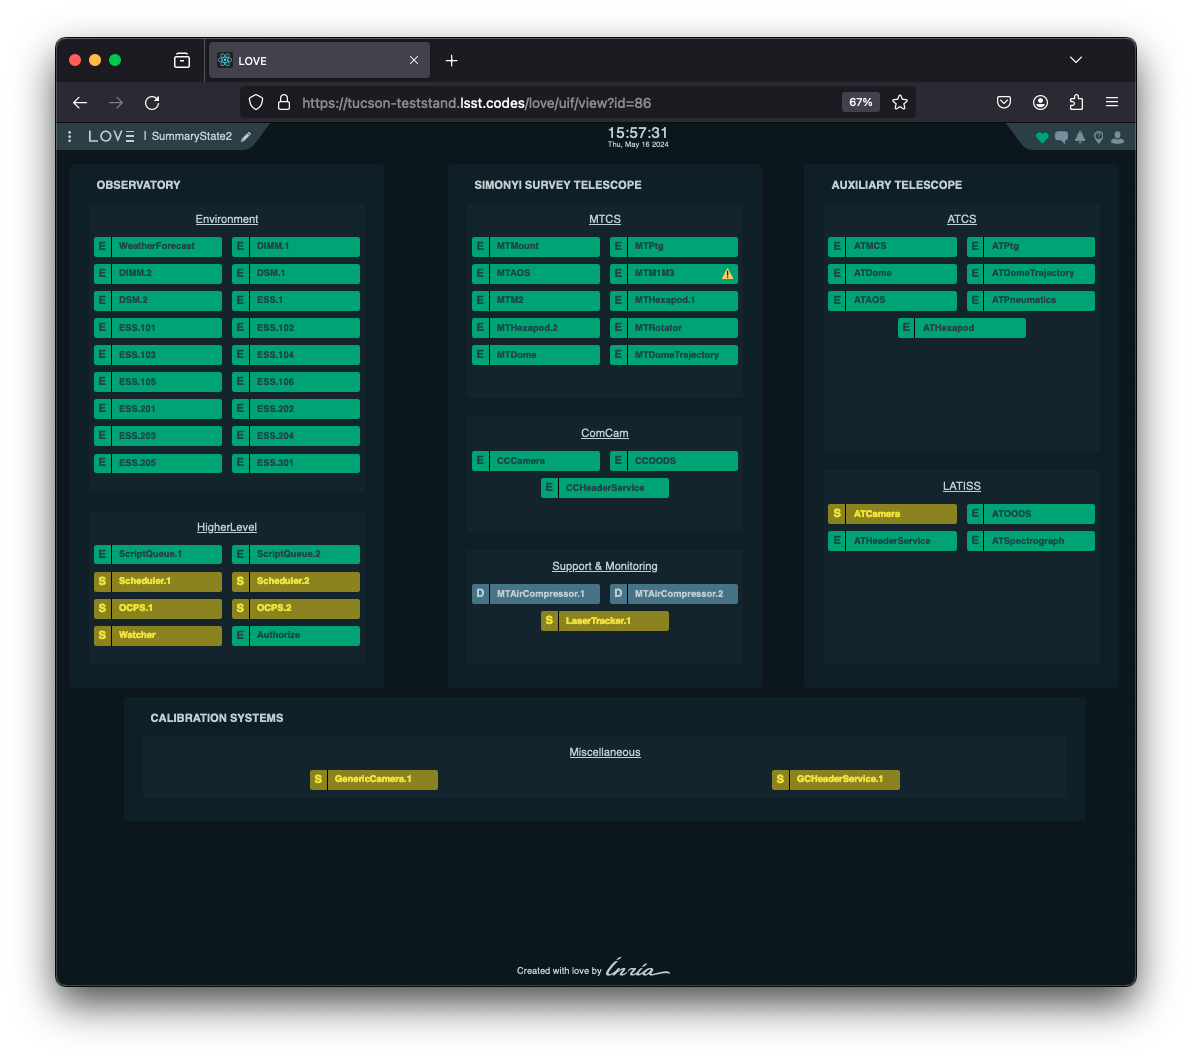
\includegraphics[width=0.3\textwidth]{figures/swd1.png}
  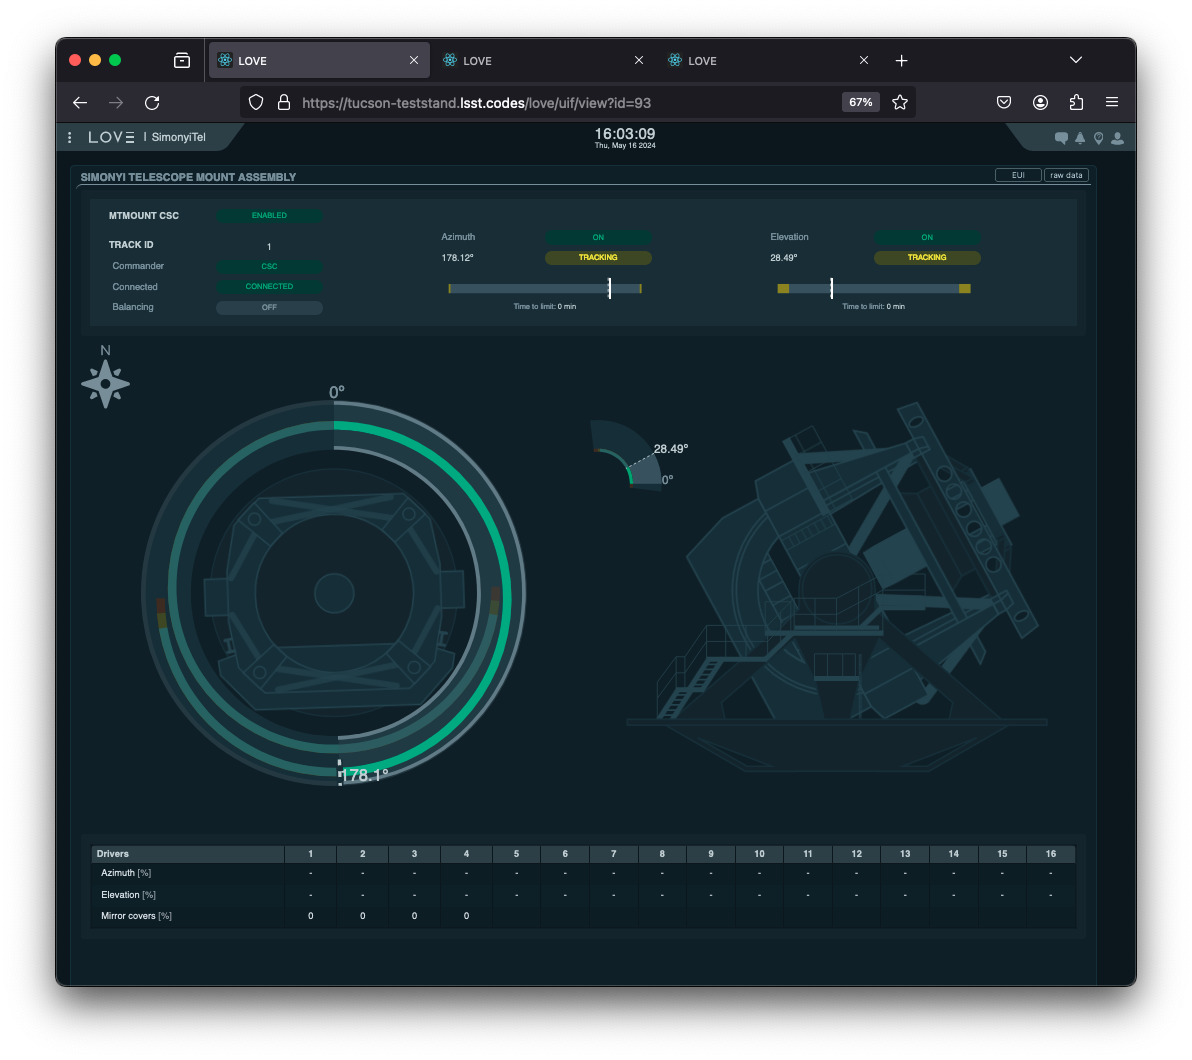
\includegraphics[width=0.3\textwidth]{figures/swd2.png}
  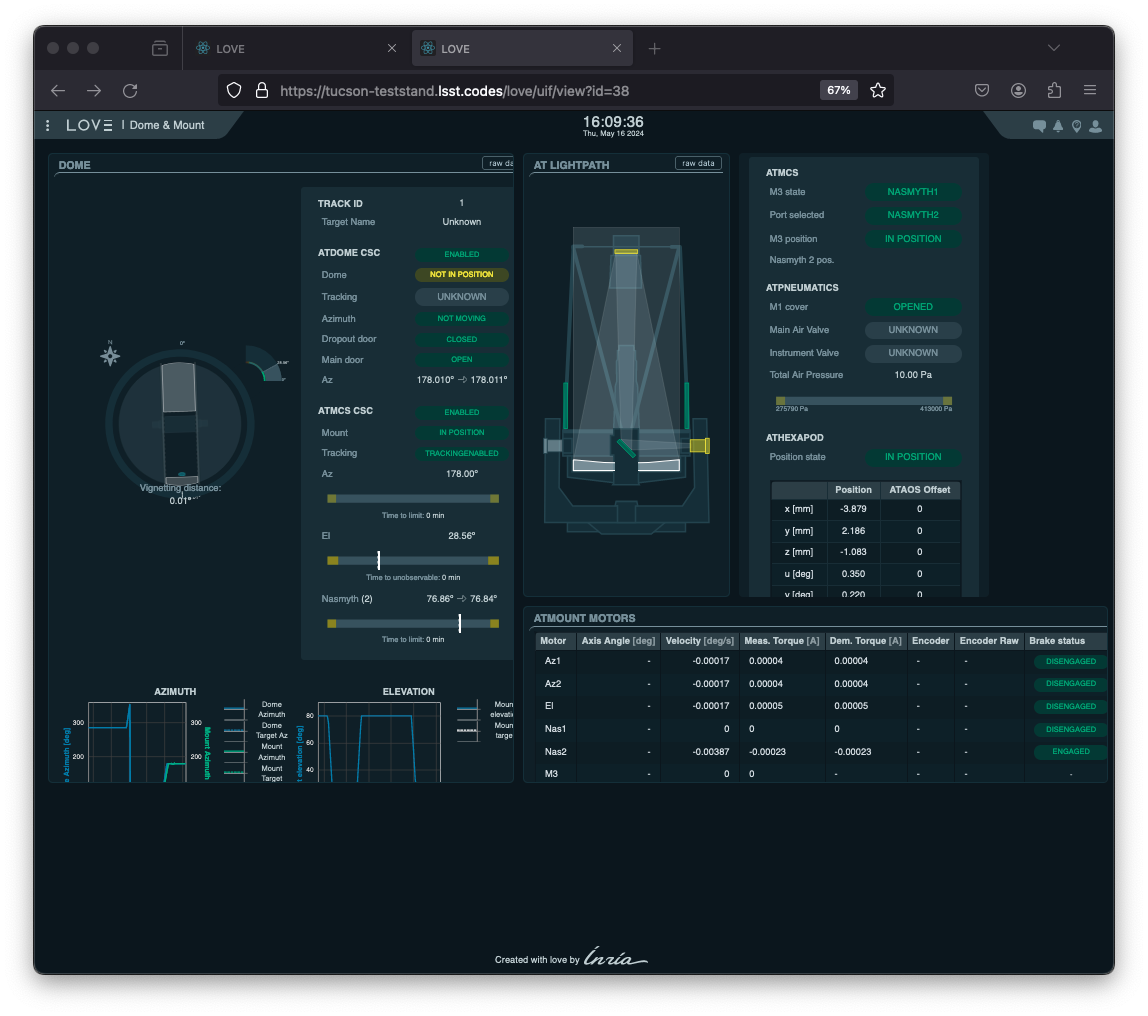
\includegraphics[width=0.3\textwidth]{figures/swd3.png}
  \caption{
    Screenshot of some of the main views of the LSST Operator Visualization Environment (LOVE) for the system running on Kafka at the Tucson Test Stand (TTS).
    The left hand panel shows the state of all the components currently running; green means the system is in Enabled state which is when they are operational, yellow systems are in Standby which means the system is alive but not able to perform any action and blue means the system is in Disable which means the system is configured and ready to operate but will not perform any action.
    Two states are not represented; Offline and Fault, which are states for components that are not running or when they experience unexpected behavior.
    The middle panel shows the view of the Simonyi telescope status, showing the current position of the telescope and the state of the different axis.
    The right hand panel show the same view for the Auxiliary Telescope.
  }\label{fig:swd}
\end{figure}


\section{Conclusions}
\label{sec:conclusions}

We have demonstrated the feasibility of replacing DDS with Kafka as the middleware technology for the Rubin-OCS.
Our initial latency and throughput benchmarks have given us confidence in implementing the update, and our Service Abstraction Layer facilitated the overall process.
We have started to execute more system-wide testing on one of our test stands, which have allowed us to gain more confidence and experience with the system.
Migration to the new Kafka-based system is expected to happen in the near future once testing has concluded and the commissioning schedule allows it.
Once migration is complete we plan to take advantage of schema evolution capabilities enabled by Kafka to improve rollout of components interfaces, reducing some of the burden on configuration management imposed by DDS.

\acknowledgments

This material is based upon work supported in part by the National Science Foundation through Cooperative Agreement AST-1258333 and Cooperative Support Agreement AST-1202910 managed by the Association of Universities for Research in Astronomy (AURA), and the Department of Energy under Contract No. DE-AC02-76SF00515 with the SLAC National Accelerator Laboratory managed by Stanford University.
Additional Rubin Observatory funding comes from private donations, grants to universities, and in-kind support from LSSTC Institutional Members.

% References
\bibliography{report} % bibliography data in report.bib
\bibliographystyle{spiebib} % makes bibtex use spiebib.bst

\end{document}

